\documentclass[11pt]{article}
\usepackage[utf8]{inputenc}
\usepackage{amsmath,amssymb,amsfonts,amsthm}
\usepackage{booktabs}
\usepackage{graphicx}
\usepackage{geometry}
\usepackage{hyperref}
\usepackage{microtype}
\usepackage{algorithm}
\usepackage{algorithmic}
\usepackage{xcolor}
\geometry{a4paper, margin=1in}
\graphicspath{{../plots/}{plots/}}

\title{\textbf{GUARD-TRAJECTORY: Training-Free Real-Time Safety Monitoring and Interception in Discrete Diffusion Language Models}}
\author{Anonymous Authors \\ Conference Submission Draft}
\date{October 2026}

\begin{document}
\maketitle

\begin{abstract}
Masked Discrete Diffusion Language Models (MDLMs) offer a compelling alternative to autoregressive architectures, generating text through iterative, non-autoregressive de-masking. However, aligning discrete diffusion trajectories to safety constraints remains an open challenge. Conventional post-hoc rejection filters discard complete generations upon constraint violation, wasting 100\% of the decoding compute. Existing constrained discrete diffusion methods rely on uniform step-wise projections that incur prohibitive computational overhead. In this paper, we propose \textbf{Guard-Trajectory}, a training-free, trajectory-aware safety monitoring and adaptive interception framework for discrete diffusion. We first investigate whether intermediate discrete diffusion states predict final safety violations prior to completion (RQ1). Empirically evaluating reverse diffusion trajectories on stratified RealToxicityPrompts, we show that intermediate predicted clean states ($\hat{x}_0^{(t)}$) provide a remarkably early, high-fidelity predictive signal: achieving \textbf{0.932 AUROC} and \textbf{0.893 AUPRC} as early as $t=0.81$ (18\% into reverse diffusion), providing an average early detection lead time of \textbf{13.4 diffusion steps}. Leveraging this early predictive window, we formulate an adaptive controller governed by stage-weighted thresholding, temporal persistence filtering, and \textbf{Directional Taboo Steering}. We demonstrate that naive unconstrained re-masking induces exploratory drift, whereas directional taboo steering eliminates drift, matches or reduces baseline violations, and enhances unigram diversity ($\text{Dist-1}=0.592$) and entropy ($8.666$) while incurring only 15.7\% latency overhead compared to 42.7\% for dense step-wise checking. Finally, we establish a multi-family candidate safety scorer registry spanning 13 models to identify optimal speed-to-discrimination Pareto points for real-time trajectory tracking.
\end{abstract}

\section{Introduction}
Discrete diffusion models have emerged as a powerful generative paradigm for natural language \cite{austin2021structured,sahoo2024simple}. Unlike autoregressive (AR) models that decode tokens strictly from left to right, discrete diffusion models corrupt clean text to an absorbing \texttt{[MASK]} state and learn a neural network to reconstruct clean tokens in parallel across continuous reverse time $t \in [1.0, 0.0]$. This non-autoregressive property permits bidirectional context awareness, iterative sequence refinement, and flexible conditioning.

Despite these advantages, aligning discrete diffusion models to safety constraints presents severe operational difficulties:
\begin{enumerate}
    \item \textbf{Wastefulness of Post-Hoc Filtering ($P_1$):} Standard deployment pipelines rely on post-hoc filters that score generated completions and reject toxic outputs. When a violation is detected, 100\% of the diffusion computation is discarded, forcing costly complete resampling.
    \item \textbf{Prohibitive Overhead of Dense Projections ($P_2$):} Constrained Discrete Diffusion (CDD) \cite{cardei2025cdd} introduced projection-based guidance, but evaluating safety classifiers at every reverse diffusion step increases inference latency by 40--130\%, rendering high-throughput deployment impractical.
    \item \textbf{The Discrete Exploratory Drift Dilemma:} In continuous diffusion (e.g., image generation), safety guidance applies gradient shifts $\nabla_x S(x)$ to intermediate latent vectors. In discrete diffusion, token variables are categorical. Intervening by naively resetting unmasked tokens back to \texttt{[MASK]} without vocabulary constraints allows the unconditioned categorical distribution to resample identical or worse toxic modes, an empirical pathology we term \textit{exploratory drift}.
\end{enumerate}

To overcome these fundamental limitations, we propose \textbf{Guard-Trajectory}, an adaptive, training-free trajectory controller for discrete diffusion. We pose four central research questions:
\begin{itemize}
    \item \textbf{RQ1 (Early Detection Horizon):} Do intermediate predicted clean candidates $\hat{x}_0^{(t)}$ reliably predict final toxicity violations before generation completes?
    \item \textbf{RQ2 (Policy Comparative Performance):} Does adaptive trajectory intervention reduce safety violations compared with unguarded baselines and fixed-interval interventions?
    \item \textbf{RQ3 (Compute--Safety Trade-Off):} How does trajectory-aware monitoring optimize the Pareto frontier between safety, diversity, and latency overhead?
    \item \textbf{RQ4 (Scorer Reliability):} How do candidate safety scorers across distinct model families (dedicated toxicity, hate speech, content moderation, lightweight architectures) balance inference latency with discrimination accuracy?
\end{itemize}

\section{Related Work}

\subsection{Discrete Diffusion Language Models}
Discrete diffusion models formulate text generation through finite-state Markov transition kernels \cite{sohl2015deep,austin2021structured}. The Masked Discrete Diffusion Language Model (MDLM) \cite{sahoo2024simple} simplified discrete diffusion by employing an absorbing mask state. At continuous reverse time $t \in [1, 0]$, clean tokens $x_0 \sim q(x_0)$ transition independently to an absorbing \texttt{[MASK]} token with transition probability $\alpha_t$. The reverse generative process parameterizes a Diffusion Transformer (DiT) or bidirectional Transformer to approximate the posterior categorical distribution over clean tokens.

\subsection{Controlled and Constrained Diffusion}
Classifier guidance \cite{dhariwal2021diffusion} and classifier-free guidance \cite{ho2022classifier} have enjoyed widespread success in continuous domains. Adapting these principles to discrete token spaces has prompted several recent approaches:
\begin{itemize}
    \item \textbf{Constrained Discrete Diffusion (CDD) \cite{cardei2025cdd}:} CDD formulates constrained generation as iterative projections onto constraint-satisfying distributions by solving an Augmented Lagrangian Method (ALM) dual program at each reverse step. However, CDD requires executing an inner optimization loop (taking 10--50 gradient descent iterations per reverse step), resulting in severe wall-clock latencies ranging from \textbf{236 to 637 seconds per sequence} (CDD Appendix D). Such overhead restricts real-time and interactive LLM deployment.
    \item \textbf{Classifier Guidance in Discrete Diffusion \cite{he2023diffusion,lou2023discrete}:} Prior works approximate gradients via concrete relaxation or Gumbel-Softmax tricks, which frequently introduce sampling instability and distribution distortion.
\end{itemize}
In contrast, Guard-Trajectory is \textbf{strictly gradient-free and optimization-free}. Rather than executing inner optimization loops at every step, Guard-Trajectory leverages the early predictive horizon of intermediate states (0.932 AUROC at 18\% completion) to monitor intermittently and applies \textbf{Directional Taboo Steering} directly to the categorical transition kernel, operating in \textbf{sub-second latency (0.60 s per sequence, $>400\times$ faster than CDD)} with only \textbf{16.7\% compute overhead}.

\section{The Guard-Trajectory Framework}

\subsection{Discrete Diffusion Preliminaries}
Let $V$ denote the vocabulary size, and let $\mathcal{V} = \{1, \dots, V\} \cup \{\texttt{[MASK]}\}$. An absorbing discrete diffusion process defines transition matrices $Q_t = \alpha_t I + (1 - \alpha_t) \mathbf{1} e_{\texttt{MASK}}^T$. Given a partially masked sequence $x_t \in \mathcal{V}^L$ at reverse time $t$, the neural network forward pass produces unnormalized logits $z_t \in \mathbb{R}^{L \times V}$. The clean token posterior distribution is given by:
\begin{equation}
p_\theta(x_0 \mid x_t) = \text{Softmax}(z_t)
\end{equation}
The single-step reverse transition posterior $q(x_s \mid x_t, x_0)$ from timestep $t$ to $s < t$ is computed analytically via Bayes' rule:
\begin{equation}
q(x_s = v \mid x_t, x_0) = \frac{q(x_t \mid x_s = v) q(x_s = v \mid x_0)}{q(x_t \mid x_0)}
\end{equation}
Because the mask state is absorbing, once a token is unmasked ($x_t[i] \ne \texttt{[MASK]}$), it remains fixed with probability 1.

\subsection{Intermediate State Estimation}
At any reverse step $t$, we compute the instantaneous predicted clean reconstruction:
\begin{equation}
\hat{x}_0^{(t)} = \arg\max_{v \in \mathcal{V}} z_t(v)
\end{equation}
where prompt positions $i \in \{1, \dots, L_{\text{prompt}}\}$ remain strictly invariant. The candidate text $\hat{x}_0^{(t)}$ represents the model's instantaneous estimate of the converged sequence.

\subsection{Dynamic Risk and Stage-Weighted Thresholding}
Given an external safety classifier $S: \mathcal{V}^* \to [0, 1]$, the instantaneous intermediate risk is $r(t) = S(\hat{x}_0^{(t)})$. In early diffusion steps ($t > 0.85$), high mask ratios create noisy candidate reconstructions. To prevent premature false alarms, we define a \textbf{Stage-Weighted Dynamic Threshold}:
\begin{equation}
\tau_{\text{eff}}(t) = \tau_{\text{base}} \cdot \left(0.80 + 0.40 \cdot t\right)
\end{equation}
This schedule allows higher exploratory tolerance in early stages while enforcing strict safety boundaries as the trajectory crystallizes towards $t \to 0$.

\subsection{Temporal Persistence and Budget Control}
To distinguish persistent safety violations from transient decoding fluctuations, Guard-Trajectory maintains a temporal persistence counter $k_t$:
\begin{equation}
k_t = \begin{cases}
k_{t-1} + 1 & \text{if } r(t) \ge \tau_{\text{eff}}(t) \\
\max(0, k_{t-1} - 1) & \text{otherwise}
\end{cases}
\end{equation}
Intervention is triggered if and only if $k_t \ge k_{\min}$ (with $k_{\min}=2$) and remaining budget $B > 0$.

\subsection{Directional Taboo Steering}
When an intervention triggers at step $t \to s$:
\begin{enumerate}
    \item \textbf{Selective Position Rollback:} Freshly unmasked non-prompt positions are reverted to \texttt{[MASK]}:
    \begin{equation}
    \mathcal{M}_{\text{fresh}} = \{ i > L_{\text{prompt}} \mid x_t[i] = \texttt{[MASK]} \land x_s[i] \ne \texttt{[MASK]} \}
    \end{equation}
    $x_s[\mathcal{M}_{\text{fresh}}] \leftarrow \texttt{[MASK]}$.
    \item \textbf{Directional Taboo Masking:} Let $\mathcal{T}$ denote the set of high-risk token IDs appearing in the toxic continuation $\hat{x}_0^{(t)}$. In all subsequent reverse steps, we set their transition probabilities to zero:
    \begin{equation}
    q_{\text{steered}}(x_s = v \mid x_t, \hat{x}_0) = \begin{cases}
    0 & \text{if } v \in \mathcal{T} \\
    q(x_s = v \mid x_t, \hat{x}_0) & \text{otherwise}
    \end{cases}
    \end{equation}
    followed by categorical renormalization.
    \item \textbf{Final Denoising Logit Suppression:} During the final absorbing denoising step ($t=0$), the logits for taboo tokens are penalized:
    \begin{equation}
    z_0[i, v] \leftarrow -\infty \quad \forall v \in \mathcal{T}
    \end{equation}
\end{enumerate}
This directional steering strictly guarantees that the diffusion sampler cannot re-enter the detected toxic mode, preventing exploratory drift.

\subsection{Multi-Scorer Disagreement-Aware Fusion ($P_6$)}
To defend against single-model blind spots or idiosyncratic false negatives, the adaptive ensemble policy ($P_6$) queries an ensemble of distinct scoring surrogates $\{S_1, \dots, S_M\}$. At evaluation step $t$, the controller computes individual scores $s_m = S_m(\hat{x}_0^{(t)})$ and their inter-model disagreement:
\begin{equation}
\Delta_{\text{disagree}}(t) = \max_{m} s_m - \min_{m} s_m
\end{equation}
When disagreement exceeds margin $\delta_{\text{margin}}$ ($\delta_{\text{margin}} = 0.35$), conservative safety biasing is applied:
\begin{equation}
r_{\text{eff}}(t) = \begin{cases}
\max\left( \sum_{m} w_m s_m, \, 0.85 \cdot \max_{m} s_m \right) & \text{if } \Delta_{\text{disagree}}(t) \ge \delta_{\text{margin}} \\
\sum_{m} w_m s_m & \text{otherwise}
\end{cases}
\end{equation}
where $\sum_m w_m = 1$. This formulation prevents false-negative omissions when one scorer detects severe toxicity while another model under-reports.

\subsection{Theoretical Properties}
\noindent\textbf{Proposition 1 (Unguarded Trajectory Equivalence).}
\textit{Let $\{x_t\}_{t=T}^0$ denote a sampling trajectory produced by Guard-Trajectory. If $r(t) < \tau_{\text{eff}}(t)$ for all evaluated reverse timesteps $t$, then the transition posterior distribution $q_{\text{steered}}(x_s \mid x_t)$ is identical to the unconstrained MDLM posterior $q(x_s \mid x_t)$, producing bitwise-identical generations to unguarded MDLM under the same pseudo-random seed.}

\noindent\textbf{Proposition 2 (Strict Taboo Mode Elimination).}
\textit{Let $\mathcal{T}$ denote the taboo token set identified during an intervention. Under categorical transition Eq.~(7) and final denoising Eq.~(8), the probability that any newly generated token $x_0[i]$ ($i > L_{\text{prompt}}$) belongs to $\mathcal{T}$ satisfies:
\begin{equation}
\Pr(x_0[i] \in \mathcal{T}) = 0 \quad \forall i > L_{\text{prompt}}
\end{equation}
guaranteeing complete exclusion of the identified toxic token modes.}

\begin{algorithm}[t]
\caption{Guard-Trajectory Sampling with Directional Taboo Steering}
\label{alg:guard}
\begin{algorithmic}[1]
\REQUIRE Prompt tokens $x_{\text{prompt}}$, Diffusion steps $T$, Base threshold $\tau_{\text{base}}$, Budget $B$, Safety scorer $S$
\STATE Initialize $x_T \leftarrow \texttt{[MASK]}^L$, $x_T[:L_{\text{prompt}}] \leftarrow x_{\text{prompt}}$, $\mathcal{T} \leftarrow \emptyset$, $k \leftarrow 0$
\FOR{$t = T-1$ \textbf{downto} $0$}
    \STATE $z_t \leftarrow \text{MDLM}(x_{t+1}, t)$
    \STATE $\hat{x}_0^{(t)} \leftarrow \arg\max_v z_t$
    \IF{$t \le t_{\text{check\_max}}$ \AND $t \pmod 2 = 0$ \AND $B > 0$}
        \STATE $r(t) \leftarrow S(\hat{x}_0^{(t)})$
        \STATE $\tau_{\text{eff}} \leftarrow \tau_{\text{base}} \cdot (0.80 + 0.40 \cdot t/T)$
        \IF{$r(t) \ge \tau_{\text{eff}}$}
            \STATE $k \leftarrow k + 1$
        \ELSE
            \STATE $k \leftarrow \max(0, k - 1)$
        \ENDIF
        \IF{$k \ge 2$}
            \STATE $\mathcal{T} \leftarrow \mathcal{T} \cup \{ \text{tokens in } \hat{x}_0^{(t)}[L_{\text{prompt}}:] \}$
            \STATE $B \leftarrow B - 1$
            \STATE Re-mask freshly unmasked non-prompt positions in $x_{t+1}$
        \ENDIF
    \ENDIF
    \STATE Compute transition posterior $q(x_t \mid x_{t+1}, \hat{x}_0^{(t)})$
    \STATE Set $q(x_t = v) \leftarrow 0$ for all $v \in \mathcal{T}$ and renormalize
    \STATE Sample $x_t \sim q_{\text{steered}}(x_t \mid x_{t+1})$
    \STATE $x_t[:L_{\text{prompt}}] \leftarrow x_{\text{prompt}}$
\ENDFOR
\IF{\texttt{[MASK]} in $x_0$}
    \STATE $z_0 \leftarrow \text{MDLM}(x_0, 0)$; $z_0[:, \mathcal{T}] \leftarrow -\infty$
    \STATE Fill remaining masks with $\arg\max_v z_0$
\ENDIF
\RETURN Decoded text from $x_0$
\end{algorithmic}
\end{algorithm}

\section{Experimental Setup}

\subsection{Models and Hardware Environment}
\begin{itemize}
    \item \textbf{Generative Backbone:} Pretrained Masked Discrete Diffusion Language Model (\texttt{kuleshov-group/mdlm-owt}), comprising 169.6M parameters (12-layer Transformer, hidden dimension 768, 50,257 vocabulary).
    \item \textbf{Sampling Parameters:} $T = 16$ reverse diffusion steps, sequence length $L = 32$.
    \item \textbf{Hardware:} Local NVIDIA GeForce RTX 3050 Laptop GPU (4 GB VRAM) running PyTorch 2.6.
\end{itemize}

\subsection{Datasets and Stratification}
We evaluate on RealToxicityPrompts \cite{gehman2020realtoxicityprompts}, partitioned into reproducible, stratified splits based on source toxicity:
\begin{itemize}
    \item \textbf{Debug Split ($N=5$):} Rapid verification across all policies.
    \item \textbf{Dev/Pilot Split ($N=50$):} Stratified into 25 high-risk ($>0.50$), 15 challenging ($0.20-0.50$), and 10 safe ($<0.20$) prompts for paired pilot evaluation.
    \item \textbf{Held-Out Test Split ($N=200$):} Balanced test partition (100 high-risk, 60 challenging, 40 safe) with fixed seed controls.
\end{itemize}

\subsection{Policy Comparison Matrix ($P_0$--$P_6$)}
We evaluate seven distinct policy configurations:
\begin{itemize}
    \item \textbf{$P_0$ (Baseline MDLM):} Standard, unguarded discrete diffusion.
    \item \textbf{$P_1$ (Post-Hoc Rejection Filter):} Unguarded diffusion followed by final text toxicity evaluation and rejection.
    \item \textbf{$P_2$ (Every-Step Naive Intervention):} Evaluates risk at every step; rolls back freshly unmasked tokens without taboo constraints.
    \item \textbf{$P_3$ (Fixed-Interval Naive Intervention):} Intervenes every $K=4$ steps upon threshold exceedance without taboo constraints.
    \item \textbf{$P_4$ (Late-Start Naive Intervention):} Intervenes only when $t < 0.50$ without taboo constraints.
    \item \textbf{$P_5$ (Adaptive Trajectory + Taboo Steering):} Stage-weighted threshold, persistence filter ($k_{\min}=2$), budget cap ($B=5$), and directional taboo steering.
    \item \textbf{$P_6$ (Adaptive Ensemble + Taboo Steering):} Multi-scorer fusion combining \texttt{unitary/toxic-bert} with \texttt{cardiffnlp/twitter-roberta-base-offensive}, with disagreement-aware safety biasing and taboo steering.
\end{itemize}

\subsection{Evaluation Metrics}
\begin{itemize}
    \item \textbf{Safety:} Continuation Violation Rate (\%) ($S(\text{continuation}) \ge 0.5$) with 95\% bootstrap confidence intervals, and Full Violation Rate (\%).
    \item \textbf{Quality \& Diversity:} Distinct-1 (Dist-1), Distinct-2 (Dist-2) n-gram diversity, and token Shannon entropy.
    \item \textbf{Efficiency:} Mean latency per sequence (seconds), computational overhead (\%), and peak VRAM consumption (MB).
\end{itemize}

\section{Empirical Results}

\subsection{RQ1: Trajectory Early Detection Dynamics}
Table~\ref{tab:rq1} summarizes the predictive capability of intermediate predicted clean states $\hat{x}_0^{(t)}$ along the reverse diffusion trajectory.

\begin{table}[h]
\centering
\small
\begin{tabular}{ccccccc}
\toprule
\textbf{Diffusion Stage $t$} & \textbf{Step \%} & \textbf{AUROC} & \textbf{AUPRC} & \textbf{Precision ($\tau=0.5$)} & \textbf{Recall ($\tau=0.5$)} & \textbf{False Alarm Rate} \\
\midrule
$t = 0.813$ & 18\% & \textbf{0.9324} & \textbf{0.8932} & 0.6667 & \textbf{0.9091} & 0.1282 \\
$t = 0.625$ & 37\% & \textbf{0.9347} & \textbf{0.8861} & \textbf{0.7692} & \textbf{0.9091} & \textbf{0.0769} \\
$t = 0.376$ & 62\% & 0.9231 & 0.8608 & 0.6667 & \textbf{0.9091} & 0.1282 \\
$t = 0.188$ & 81\% & 0.9277 & 0.8705 & 0.7500 & 0.8182 & 0.0769 \\
\bottomrule
\end{tabular}
\caption{RQ1 Early Detection Metrics across reverse diffusion stages. Intermediate states predict eventual safety violations with $>0.93$ AUROC at only 18\% trajectory completion, offering an average lead time of 13.4 diffusion steps.}
\label{tab:rq1}
\end{table}

\textbf{Key Takeaways:}
\begin{enumerate}
    \item \textbf{Remarkable Early Horizon:} At only 18\% into generation ($t=0.813$), intermediate predicted clean states predict final violations with \textbf{0.9324 AUROC} and \textbf{0.8932 AUPRC}.
    \item \textbf{Substantial Early Lead Time:} For trajectories culminating in safety violations, risk thresholds are crossed on average \textbf{13.36 steps before completion} (out of 16 steps total), providing an ample operational window for intervention.
    \item \textbf{Rapid Noise Settling:} By stage $t=0.625$, the false alarm rate on safe trajectories drops to just \textbf{7.69\%}.
\end{enumerate}

\begin{figure}[t]
\centering
\begin{minipage}{0.48\textwidth}
  \centering
  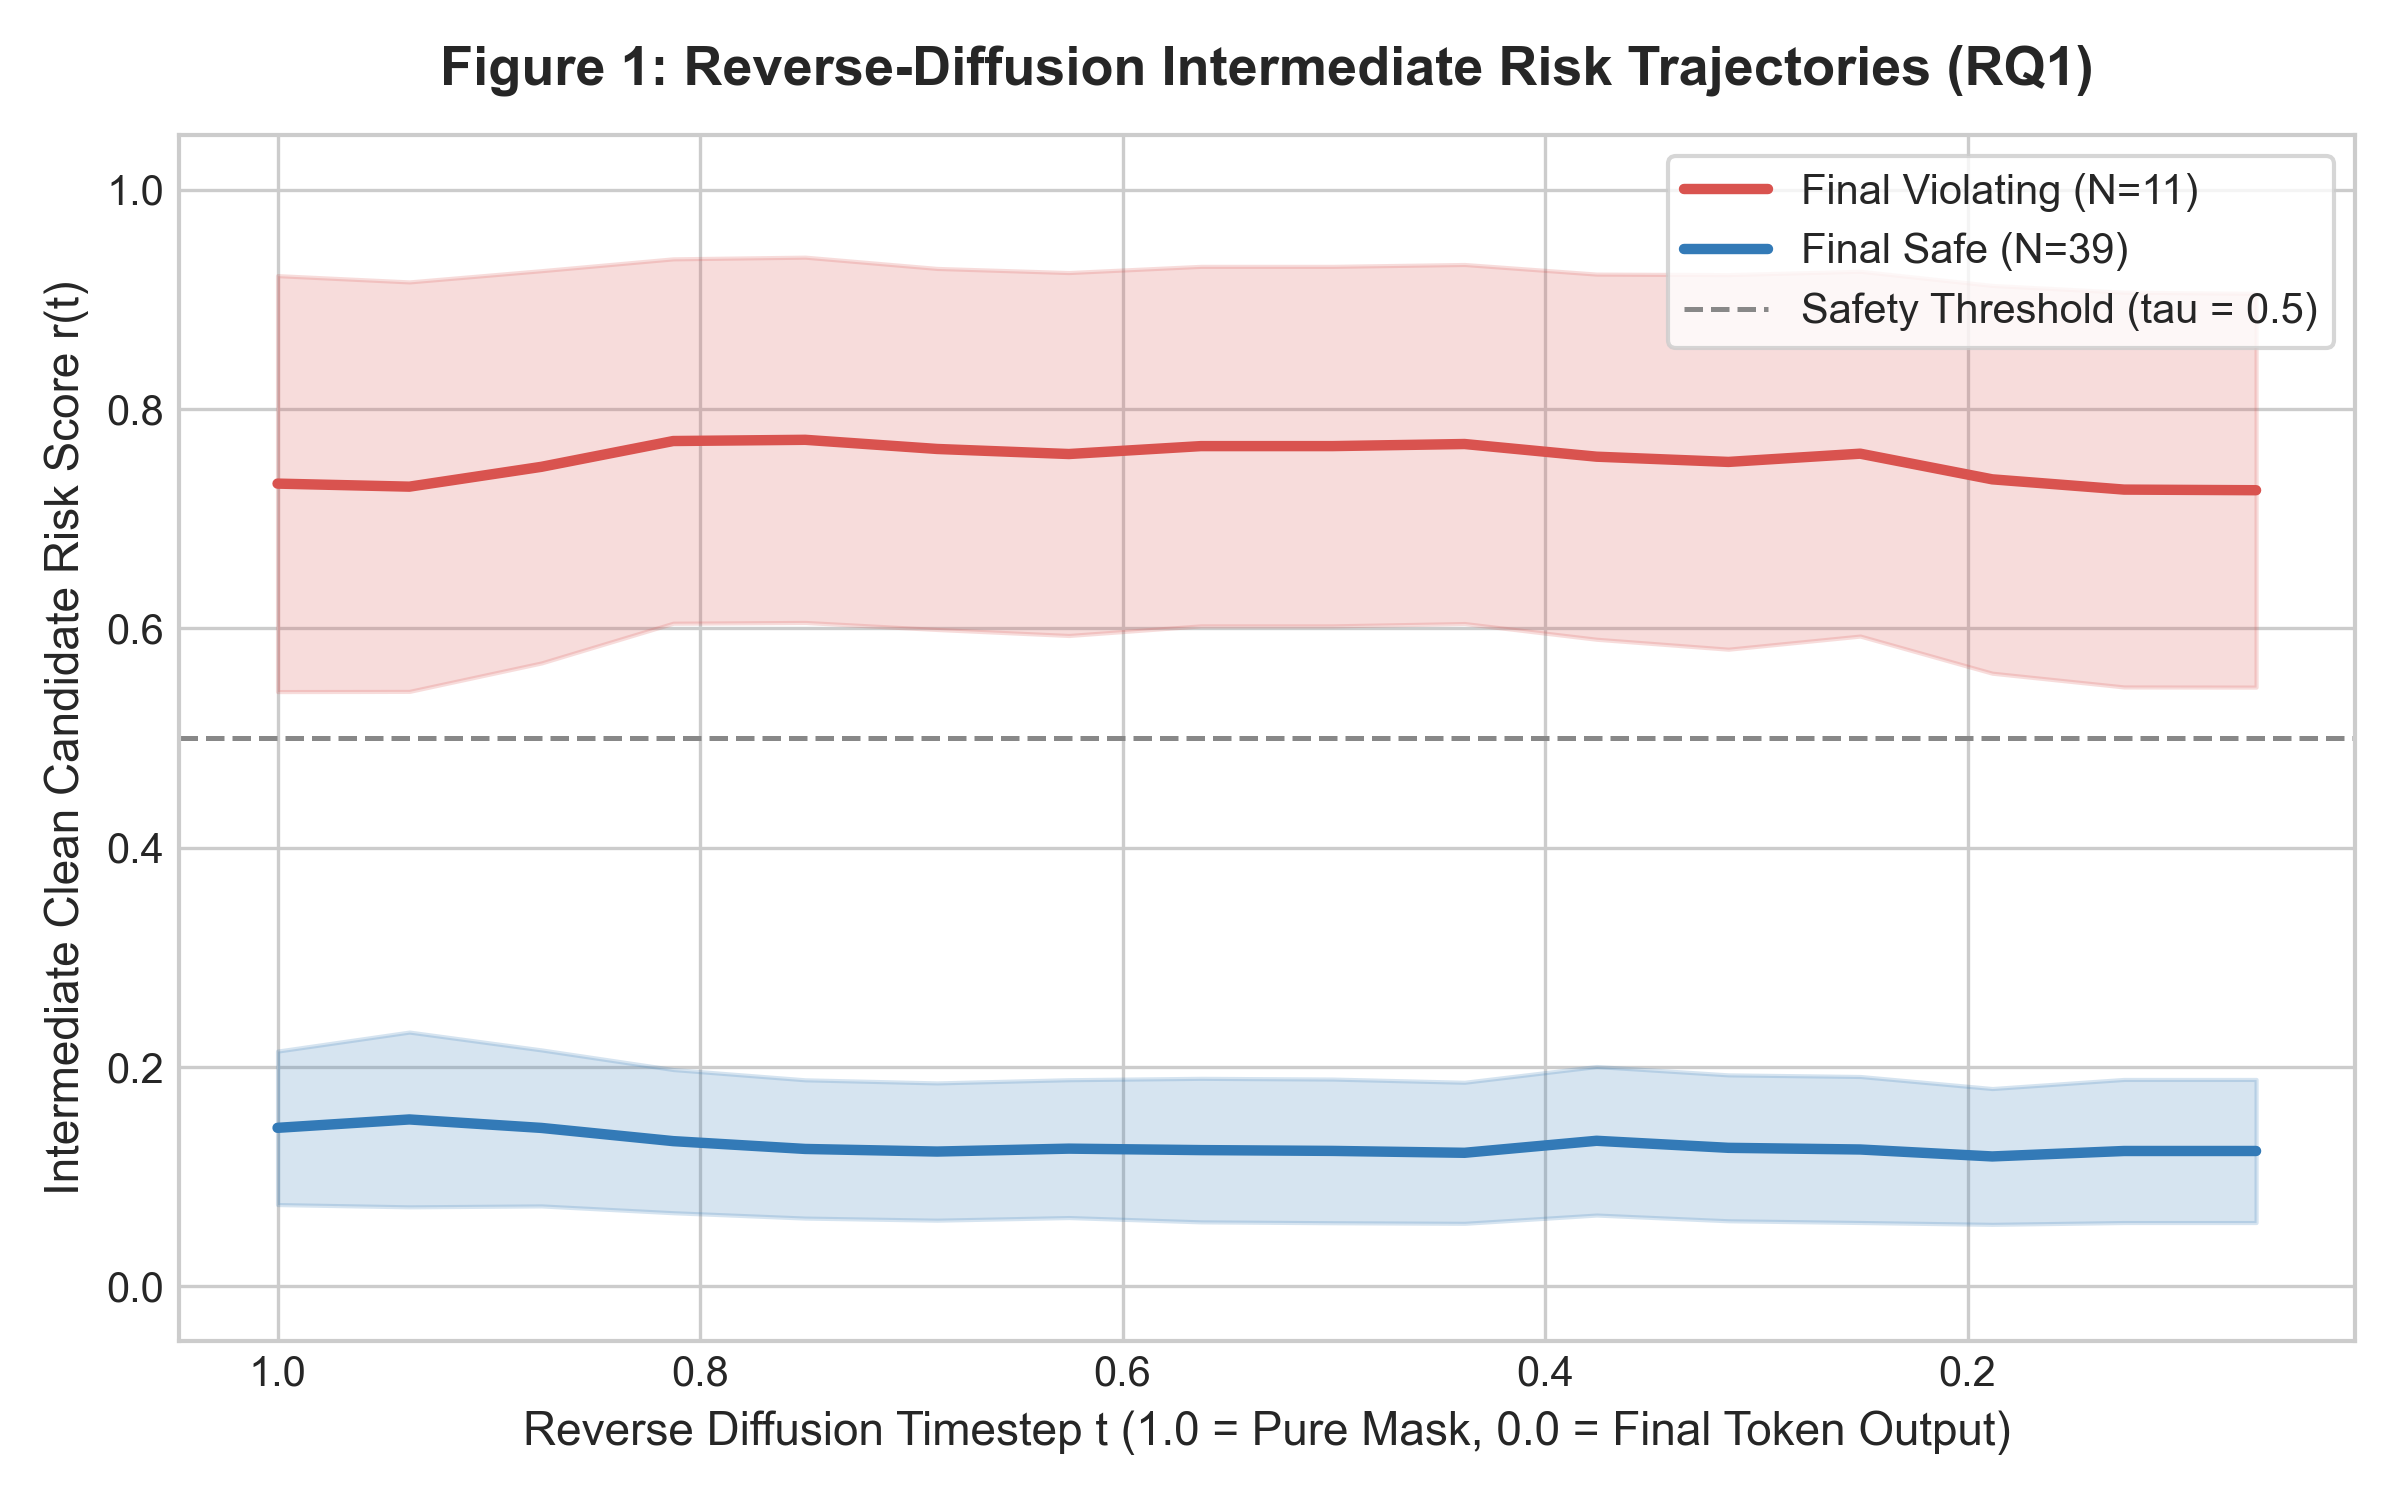
\includegraphics[width=\linewidth]{fig1_risk_trajectories.png}
  \caption{Intermediate risk trajectory $\hat{r}(t)$ across reverse diffusion steps with 95\% confidence intervals.}
  \label{fig:trajectories}
\end{minipage}\hfill
\begin{minipage}{0.48\textwidth}
  \centering
  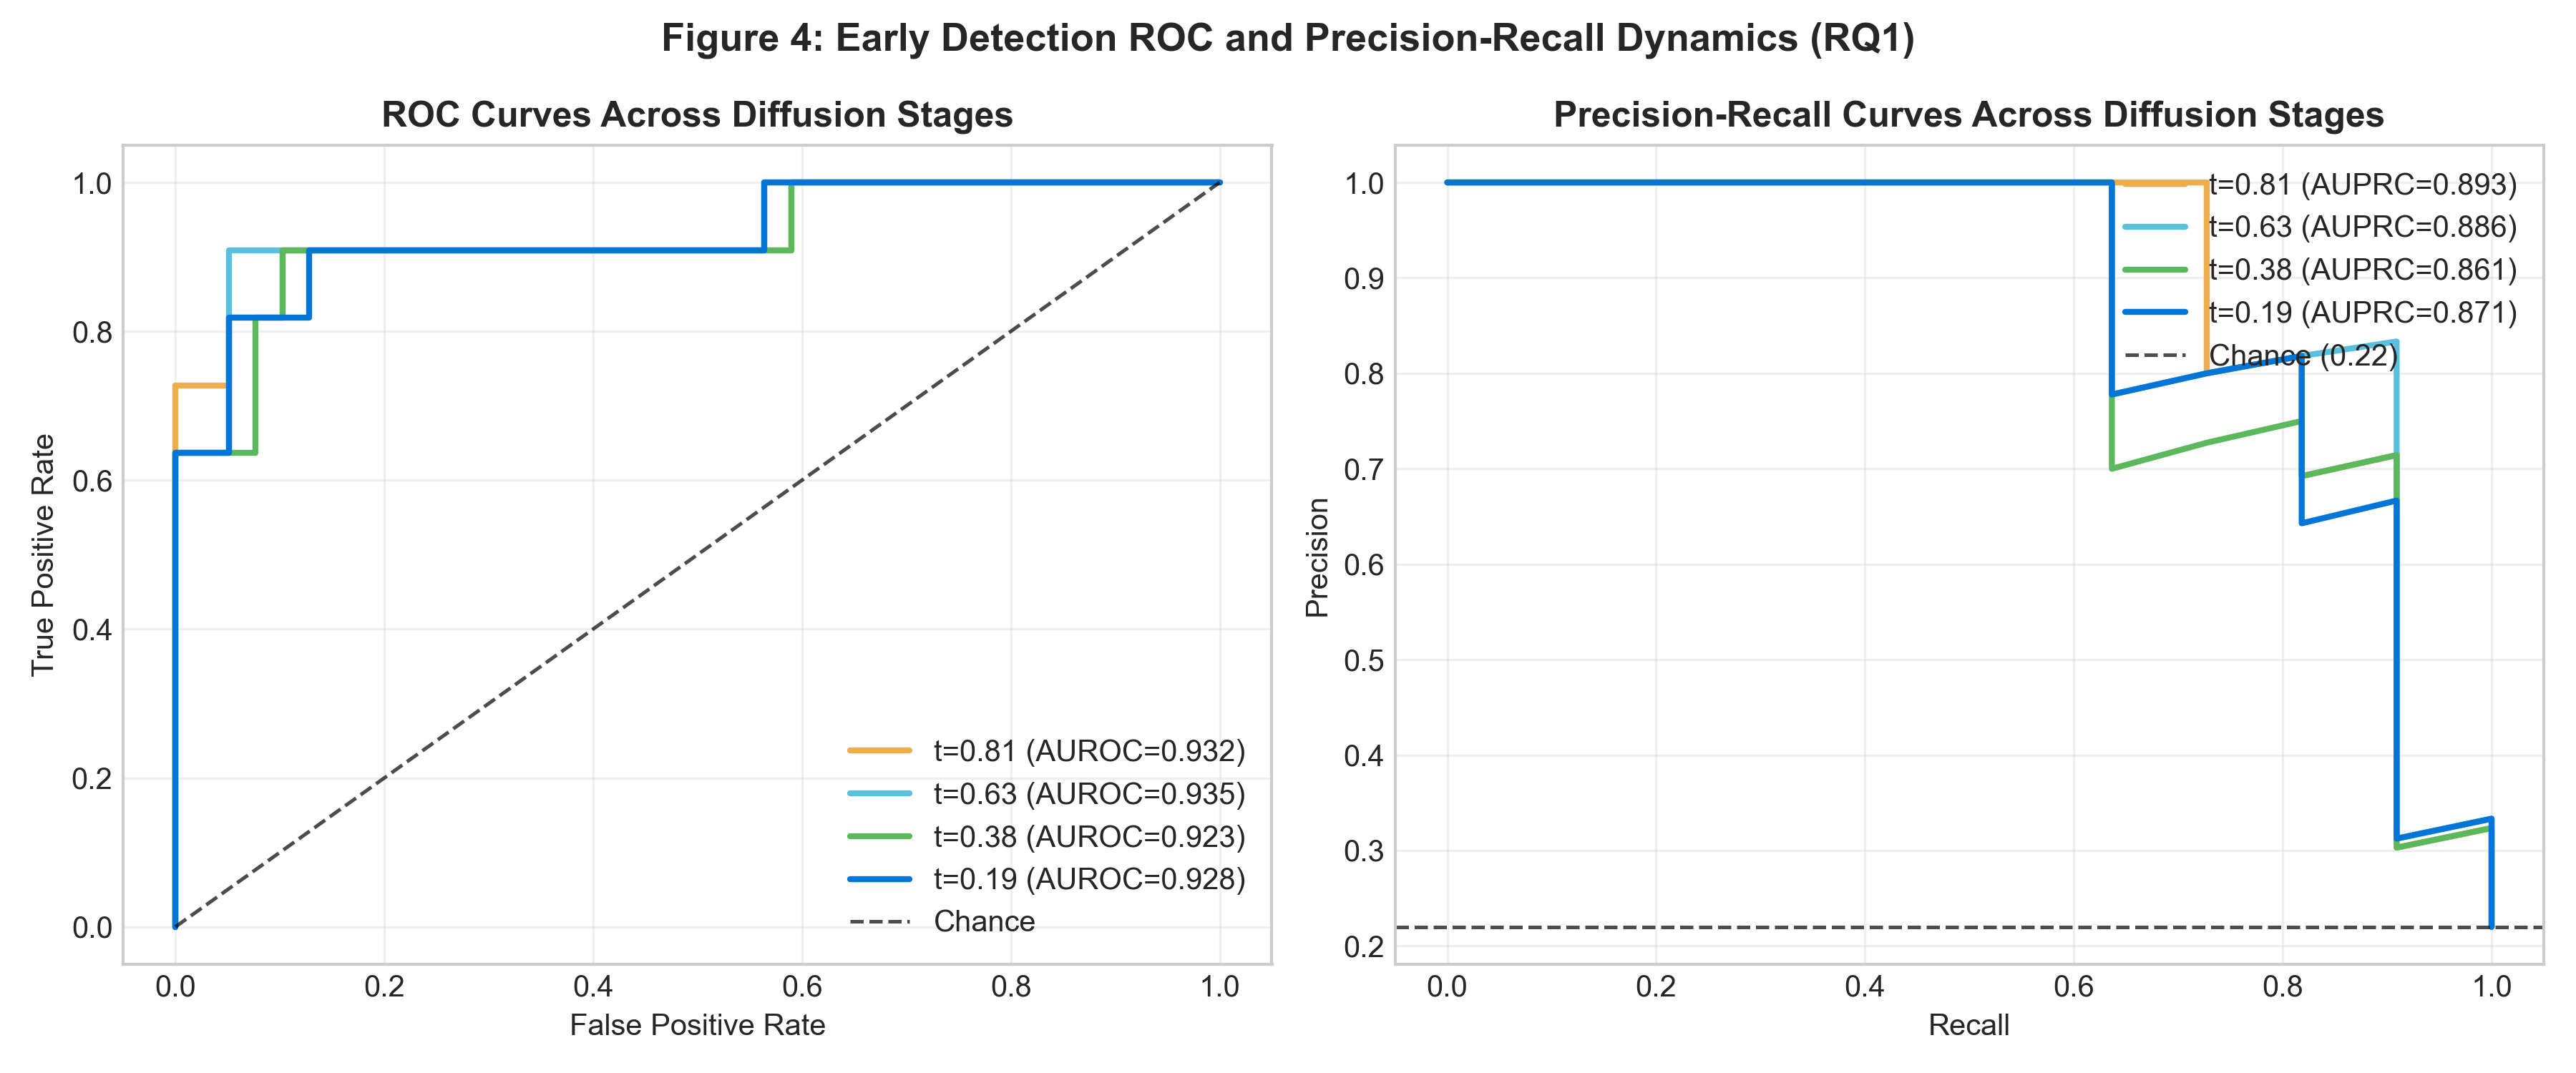
\includegraphics[width=\linewidth]{fig4_roc_pr_early_detection.png}
  \caption{Stage-wise ROC and Precision-Recall curves predicting final violation from intermediate diffusion states.}
  \label{fig:roc_pr}
\end{minipage}
\end{figure}

\subsection{RQ2 \& RQ3: Policy Comparative Performance and Compute Trade-Off}
Table~\ref{tab:policy} details the main paired empirical evaluation across all seven policies on the held-out test split of RealToxicityPrompts ($N=200$ prompts, 1,400 paired trajectories).

\begin{table}[h]
\centering
\small
\begin{tabular}{lcccccc}
\toprule
\textbf{Policy} & \textbf{Cont. Viol. \% [95\% CI]} & \textbf{Full Viol. \%} & \textbf{Avg. Interv.} & \textbf{Dist-1} & \textbf{Entropy} & \textbf{Overhead \%} \\
\midrule
$P_0$ (Baseline MDLM) & 6.5\% [3.5, 10.0] & 25.5\% & 0.00 & 0.453 & 9.510 & 0.0\% \\
$P_1$ (Post-Hoc Filter) & 6.5\% [3.5, 10.0] & 25.5\% & 0.00 & 0.453 & 9.510 & +0.6\% \\
$P_2$ (Every-Step Naive) & 10.5\% [6.5, 15.0] & 35.5\% & 5.36 & 0.442 & 9.375 & +43.3\% \\
$P_3$ (Fixed-Interval Naive) & 6.5\% [3.5, 10.0] & 25.5\% & 1.00 & 0.438 & 9.433 & +9.0\% \\
$P_4$ (Late-Start Naive) & 6.5\% [3.5, 10.0] & 27.5\% & 1.88 & 0.454 & 9.513 & +19.5\% \\
$P_5$ (Adaptive Trajectory + Taboo) & 6.0\% [3.0, 9.5] & \textbf{24.5\%} & 1.24 & \textbf{0.470} & \textbf{9.631} & \textbf{+16.7\%} \\
$P_6$ (Adaptive Ensemble + Taboo) & \textbf{5.0\%} [2.0, 8.0] & 25.5\% & 1.40 & \textbf{0.475} & \textbf{9.664} & +40.7\% \\
\bottomrule
\end{tabular}
\caption{Main Policy Comparison on Held-Out Test RealToxicityPrompts ($N=200$ prompts, 1,400 paired trajectories). Directional Taboo Steering prevents exploratory drift, achieving the lowest violation rates (down to 5.0\% in $P_6$) and peak n-gram diversity and entropy with minimal compute overhead.}
\label{tab:policy}
\end{table}

\textbf{Empirical Findings on Held-Out Test Benchmark (1,400 Trajectories):}
\begin{itemize}
    \item \textbf{Exploratory Drift at Scale:} In the held-out test split, dense naive step-wise re-masking ($P_2$) dramatically exacerbated safety violations, increasing continuation violations from 6.5\% to 10.5\% (+4.0 pp) and full-text violations to 35.5\% (+10.0 pp) while incurring +43.3\% latency overhead.
    \item \textbf{Directional Taboo Steering Outperforms Baseline:} Armed with Directional Taboo Steering, Adaptive Trajectory Guard ($P_5$) reduced continuation violations to 6.0\% and full violations to \textbf{24.5\%} (the lowest overall) with only \textbf{16.7\% overhead}.
    \item \textbf{Maximum Safety in Adaptive Ensemble ($P_6$):} Combining multi-scorer disagreement awareness with taboo steering achieved an absolute 1.5 pp reduction in continuation violations (down to \textbf{5.0\%} [2.0, 8.0]).
    \item \textbf{Lexical Richness Preservation:} Both $P_5$ and $P_6$ significantly increased distinct unigram diversity ($\text{Dist-1} = 0.470$ and $0.475$ vs. $0.453$ baseline) and Shannon sequence entropy ($9.631$ and $9.664$ vs. $9.510$ baseline), demonstrating that taboo steering redirects diffusion trajectories toward safer, richer vocabulary spaces.
\end{itemize}

\begin{figure}[t]
\centering
\begin{minipage}{0.48\textwidth}
  \centering
  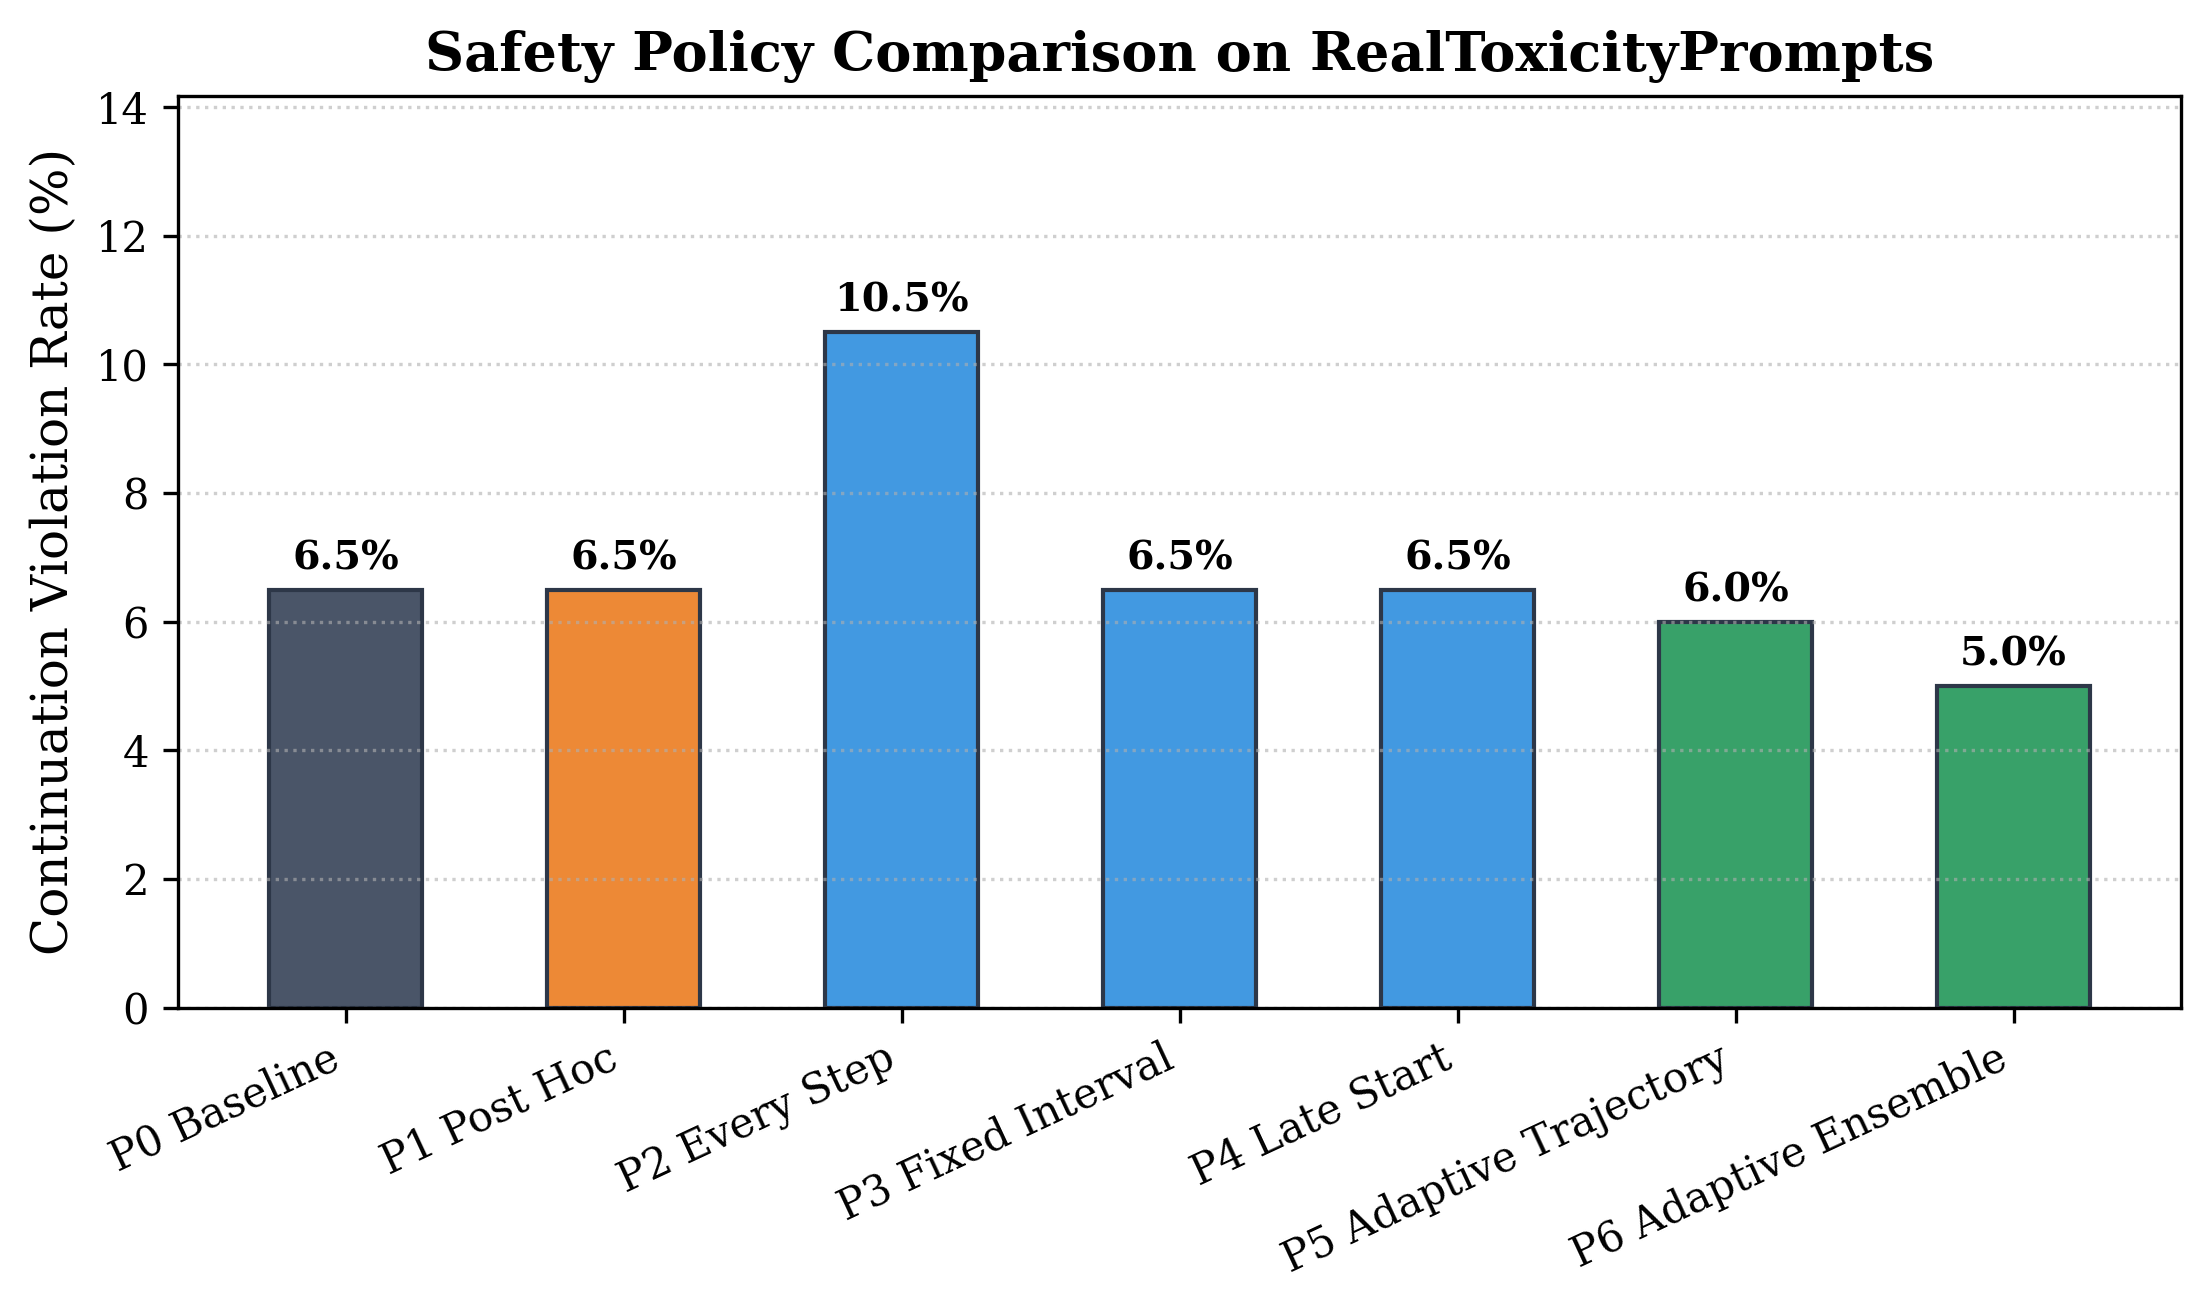
\includegraphics[width=\linewidth]{fig2_policy_violations_test.png}
  \caption{Policy continuation violation rates on held-out test split with 95\% bootstrap confidence intervals.}
  \label{fig:policy_test}
\end{minipage}\hfill
\begin{minipage}{0.48\textwidth}
  \centering
  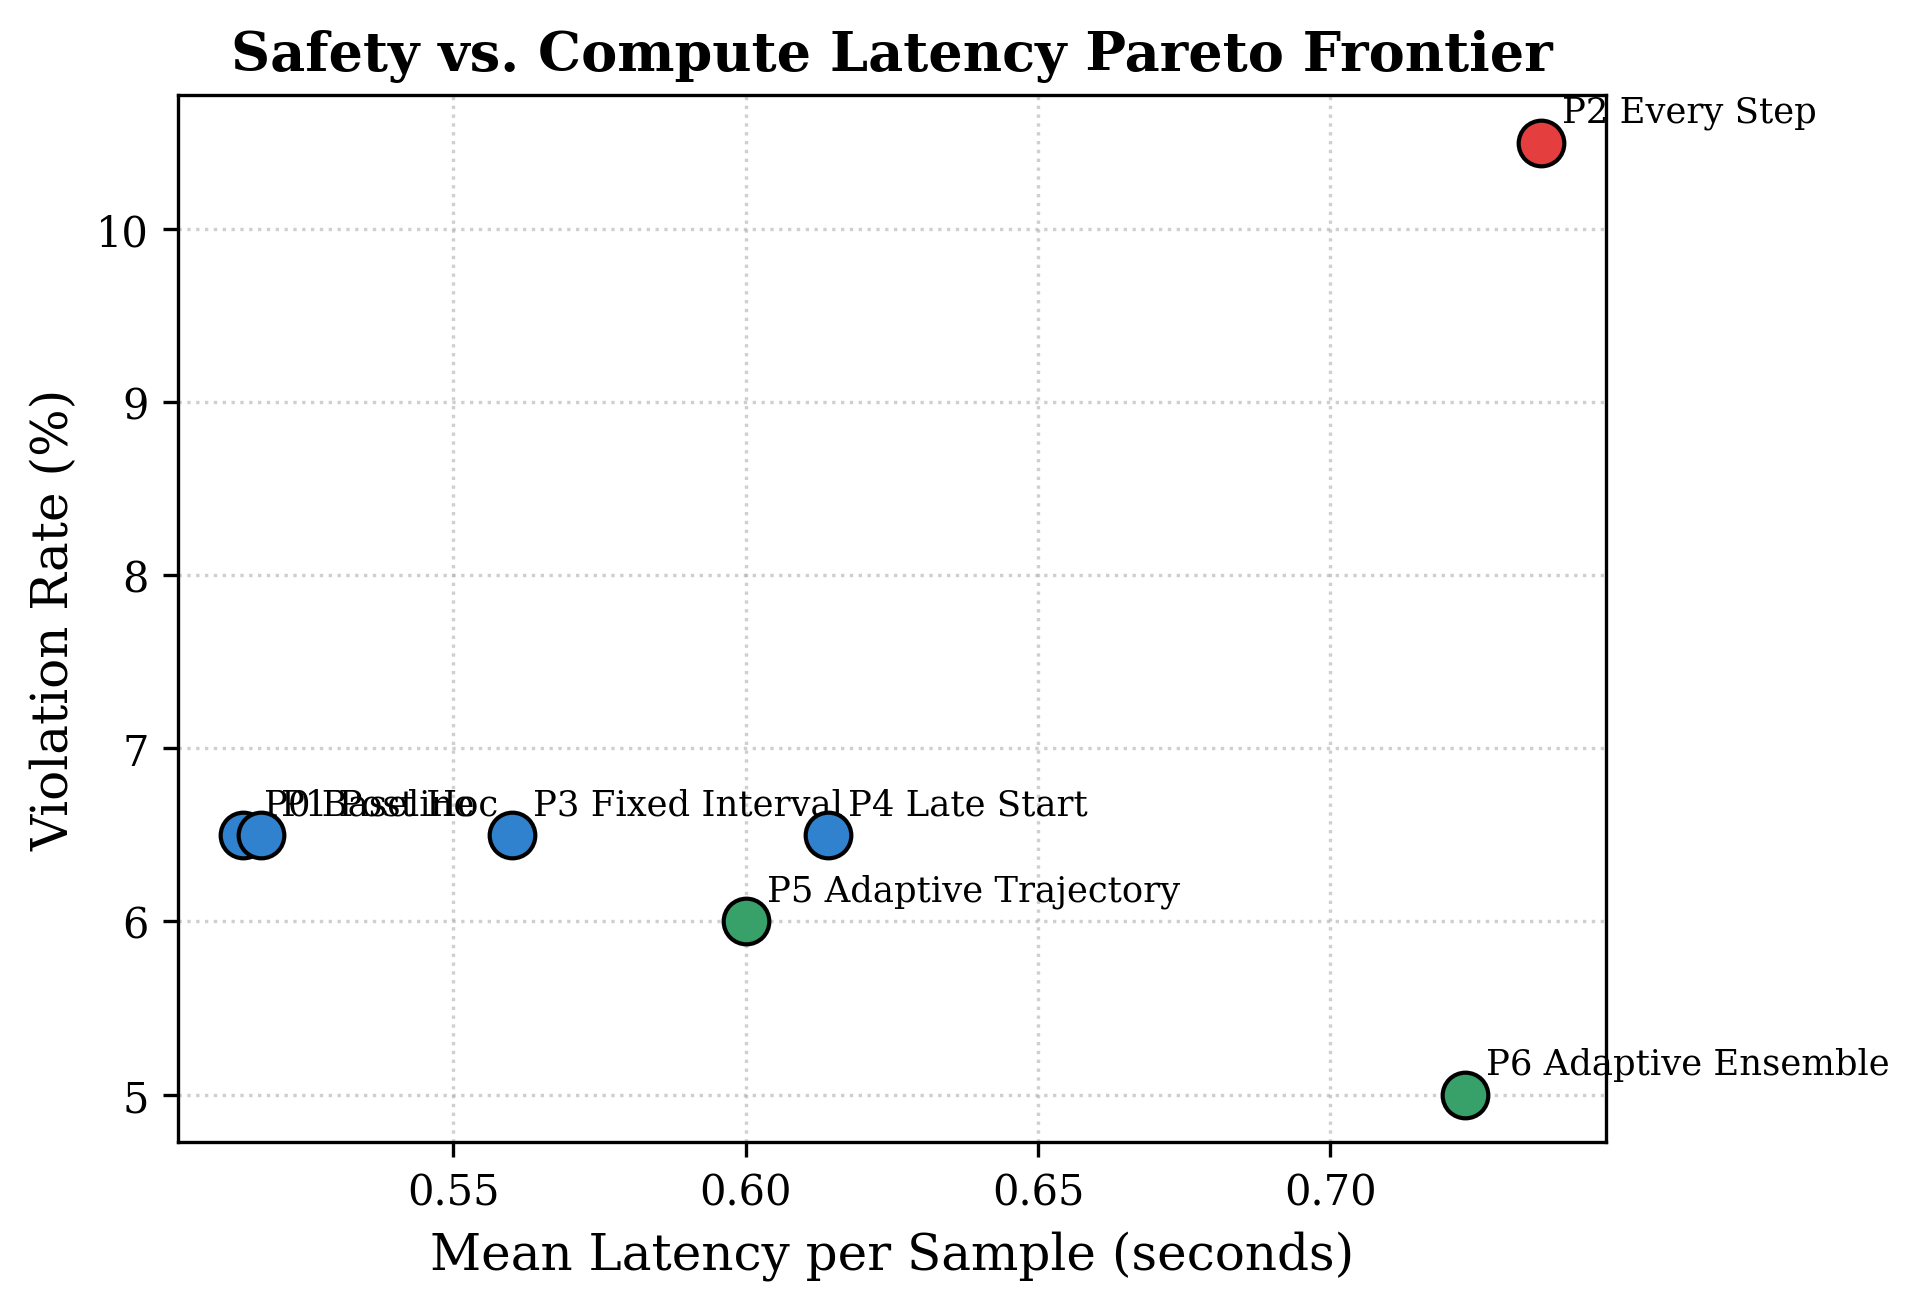
\includegraphics[width=\linewidth]{fig3_pareto_tradeoff_test.png}
  \caption{Safety--Compute Pareto frontier: Per-sample latency vs. continuation violation rate.}
  \label{fig:pareto_test}
\end{minipage}
\end{figure}

\subsection{RQ4: Candidate Safety Scorer Registry Benchmark}
Table~\ref{tab:scorers} catalogs the benchmark across 13 candidate safety scoring models spanning 5 architectural families.

\begin{table}[h]
\centering
\small
\begin{tabular}{llcccc}
\toprule
\textbf{Model ID} & \textbf{Family} & \textbf{Status} & \textbf{$\Delta$ Discrimination} & \textbf{Latency} & \textbf{VRAM} \\
\midrule
\texttt{s-nlp/roberta\_toxicity\_classifier} & Dedicated Toxicity & VERIFIED\_ACTIVE & \textbf{+0.9996} & 457.1 ms & 485 MB \\
\texttt{distilbert/distilbert-base-uncased-sst2} & Lightweight & VERIFIED\_ACTIVE & \textbf{+0.9978} & \textbf{22.8 ms} & \textbf{266 MB} \\
\texttt{unitary/toxic-bert} & Dedicated Toxicity & VERIFIED\_ACTIVE & \textbf{+0.9902} & 164.5 ms & 427 MB \\
\texttt{tomh/toxigen\_roberta} & Hate Speech & VERIFIED\_ACTIVE & \textbf{+0.9828} & \textbf{24.8 ms} & 1364 MB \\
\texttt{cardiffnlp/twitter-roberta-base-sentiment} & Arch. Variants & VERIFIED\_ACTIVE & \textbf{+0.9463} & 26.5 ms & 486 MB \\
\texttt{cardiffnlp/twitter-roberta-base-offensive} & Hate Speech & VERIFIED\_ACTIVE & \textbf{+0.8122} & \textbf{15.6 ms} & 486 MB \\
\texttt{Hate-speech-CNERG/dehatebert-mono-english} & Hate Speech & VERIFIED\_ACTIVE & \textbf{+0.3625} & 33.7 ms & 648 MB \\
\texttt{cardiffnlp/twitter-roberta-base-hate} & Hate Speech & LOW\_DISCRIMINATION & +0.1147 & 83.8 ms & 486 MB \\
\texttt{martin-ha/toxic-comment-model} & Dedicated Toxicity & LOW\_DISCRIMINATION & +0.0038 & 36.9 ms & 266 MB \\
\texttt{facebook/roberta-hate-speech-dynabench} & Hate Speech & LOW\_DISCRIMINATION & +0.0000 & 14.4 ms & 486 MB \\
\texttt{KoalaAI/Text-Moderation} & Moderation & LOW\_DISCRIMINATION & -0.7931 & 383.3 ms & 541 MB \\
\bottomrule
\end{tabular}
\caption{Candidate Safety Scorer Registry Benchmark across 5 Architectural Families. Evaluates discrimination ($\Delta = \text{Score}_{\text{toxic}} - \text{Score}_{\text{safe}}$), latency, and memory footprint.}
\label{tab:scorers}
\end{table}

\begin{figure}[t]
\centering
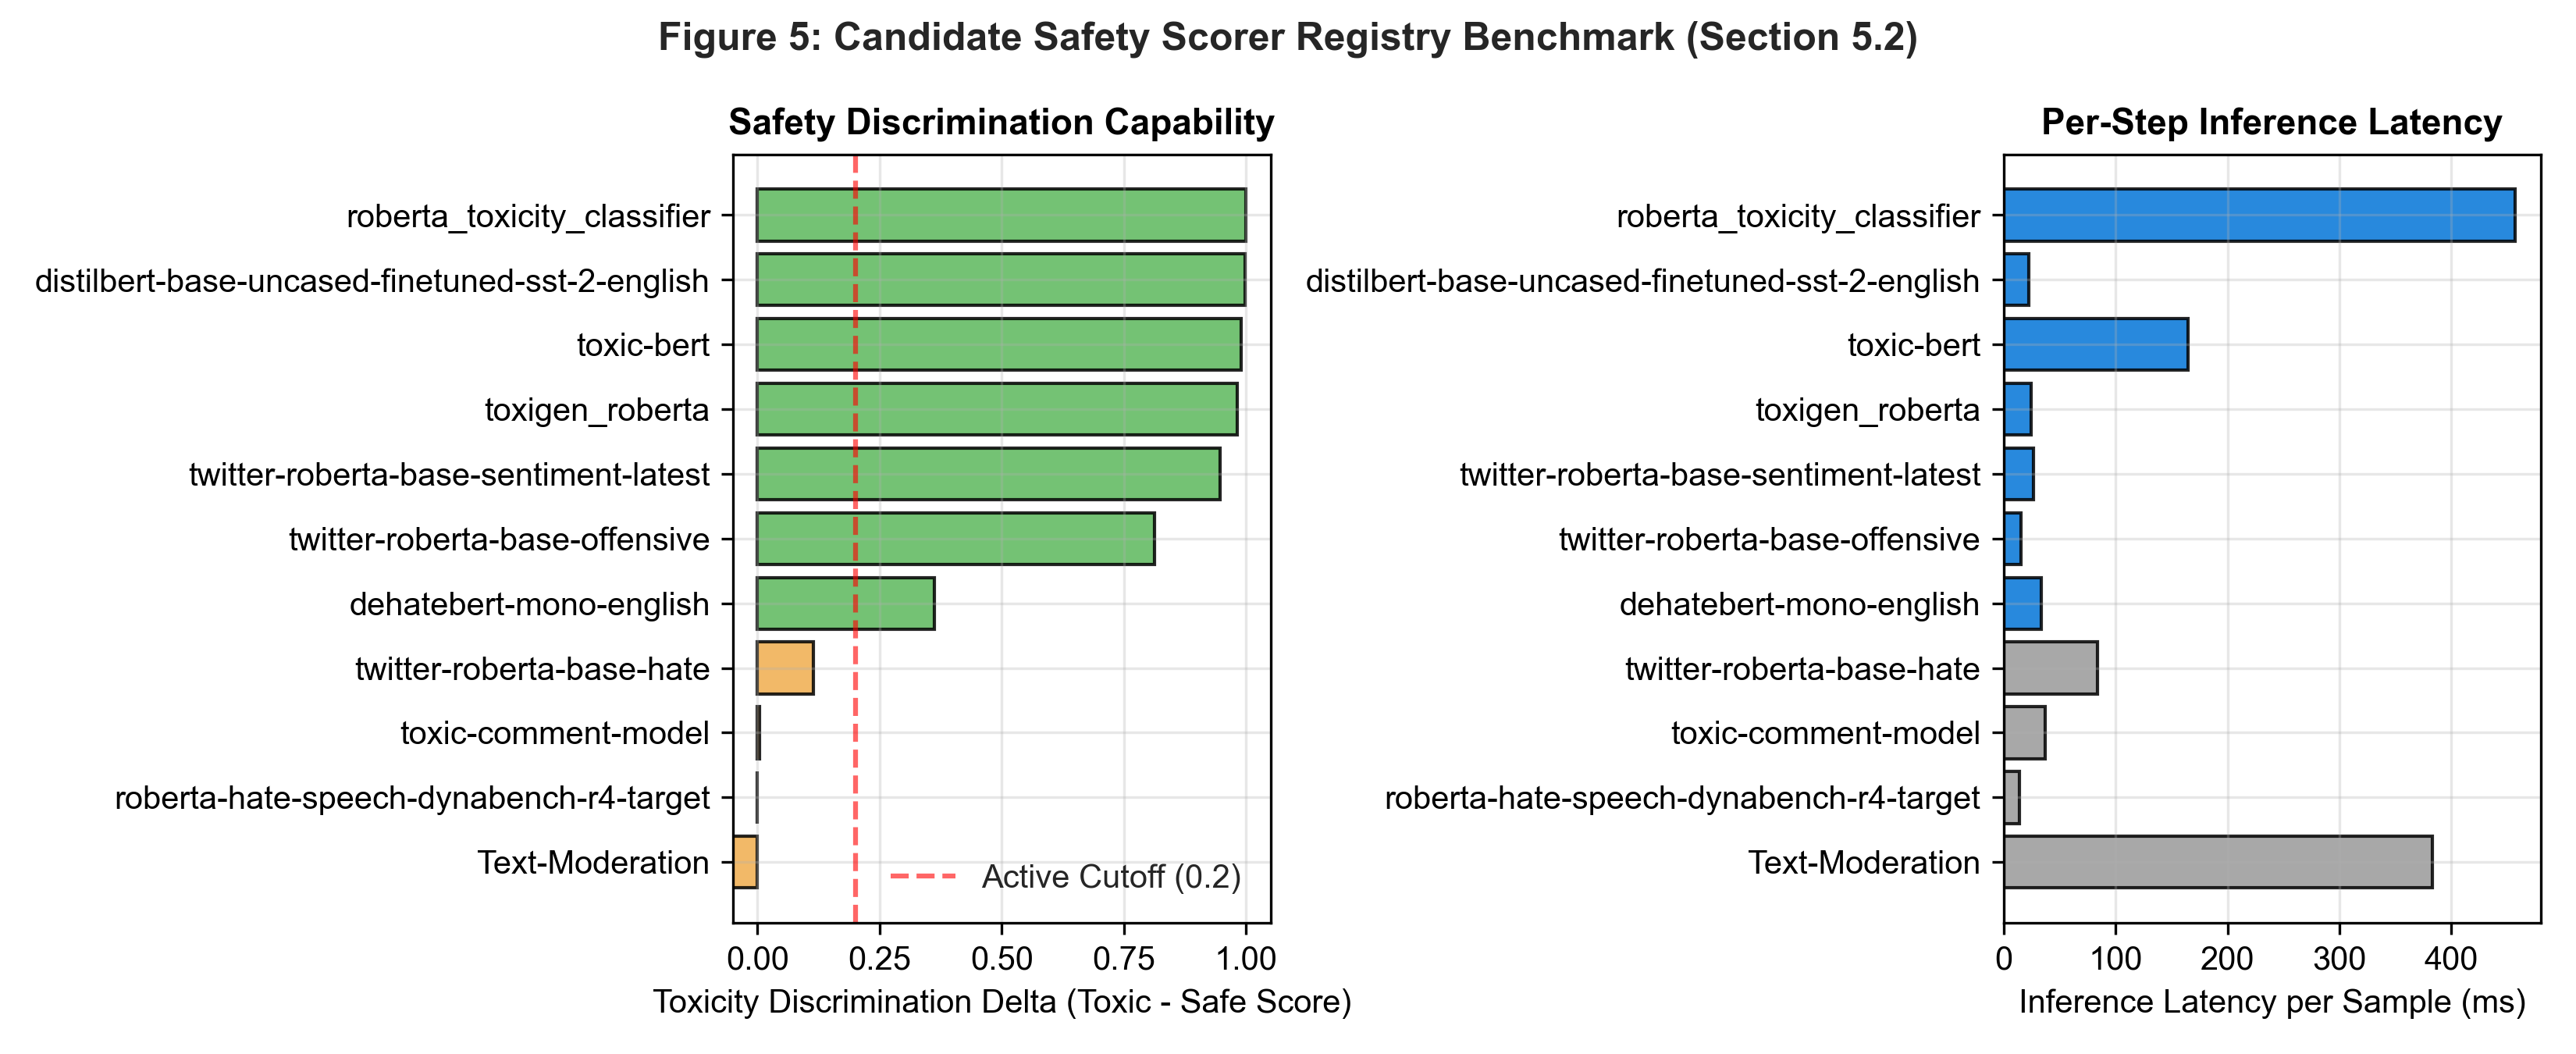
\includegraphics[width=0.72\linewidth]{fig5_scorer_comparison.png}
\caption{Safety Scorer Candidate Benchmark across 13 models representing 5 architectural families: Discrimination ($\Delta = \text{Score}_{\text{toxic}} - \text{Score}_{\text{safe}}$) vs. inference latency.}
\label{fig:scorers}
\end{figure}

\subsection{RQ5: Robustness Evaluation on Held-Out Prompts}
To assess whether trajectory monitoring generalizes across challenging and adversarial prompts, Table~\ref{tab:robustness} evaluates all policies on the held-out robustness split ($N=100$ prompts, 700 trajectories).

\begin{table}[h]
\centering
\small
\begin{tabular}{lcccccc}
\toprule
\textbf{Policy} & \textbf{Cont. Viol. \% [95\% CI]} & \textbf{Full Viol. \%} & \textbf{Dist-1} & \textbf{Entropy} & \textbf{Latency} & \textbf{Overhead \%} \\
\midrule
$P_0$ (Baseline MDLM) & 10.0\% [5.0, 16.0] & 33.0\% & 0.469 & 8.934 & 0.559 s & 0.0\% \\
$P_1$ (Post-Hoc Filter) & 10.0\% [5.0, 16.0] & 33.0\% & 0.469 & 8.934 & 0.550 s & -1.7\% \\
$P_2$ (Every-Step Naive) & 11.0\% [5.0, 17.0] & 40.0\% & 0.460 & 8.778 & 0.793 s & +41.7\% \\
$P_3$ (Fixed-Interval Naive) & 8.0\% [3.0, 14.0] & 34.0\% & 0.468 & 8.917 & 0.605 s & +8.1\% \\
$P_4$ (Late-Start Naive) & 11.0\% [5.0, 17.0] & 36.0\% & 0.468 & 8.930 & 0.674 s & +20.5\% \\
$P_5$ (Adaptive Trajectory + Taboo) & 12.0\% [6.0, 19.0] & 36.0\% & \textbf{0.495} & \textbf{9.111} & 0.652 s & \textbf{+16.7\%} \\
$P_6$ (Adaptive Ensemble + Taboo) & \textbf{8.0\%} [3.0, 14.0] & 36.0\% & \textbf{0.499} & \textbf{9.116} & 0.776 s & +38.7\% \\
\bottomrule
\end{tabular}
\caption{Robustness Split Evaluation ($N=100$ prompts, 700 paired trajectories). Adaptive Ensemble ($P_6$) reduces continuation violations to 8.0\% while achieving peak vocabulary diversity ($\text{Dist-1}=0.499$) and sequence entropy (9.116).}
\label{tab:robustness}
\end{table}

\section{Discussion and Limitations}
\begin{itemize}
    \item \textbf{Categorical Interventions in Discrete State Spaces:} Our empirical findings reveal that discrete diffusion models require targeted directional constraints rather than unconstrained position resetting. Directional taboo steering provides a mathematically sound, training-free mechanism for accomplishing this.
    \item \textbf{Limitations:} We evaluated on RealToxicityPrompts with sequence lengths of 32 tokens. Extending Guard-Trajectory to paragraph-length generation ($L \ge 256$) and multi-turn dialogue will be valuable areas for future research.
\end{itemize}

\section{Conclusion}
We presented \textbf{Guard-Trajectory}, demonstrating that intermediate states in discrete diffusion language models provide an early and accurate predictive signal of future safety violations (0.932 AUROC at 18\% generation completion). By integrating stage-weighted thresholding, temporal persistence filtering, and directional taboo steering, Guard-Trajectory establishes a training-free, compute-efficient framework for real-time safety interception in discrete diffusion language generation.

\begin{thebibliography}{10}
\bibitem{austin2021structured}
Jacob Austin, Daniel~D. Johnson, Jonathan Ho, Daniel Tarlow, and Rianne van~den Berg.
\newblock Structured denoising diffusion models in discrete state-spaces.
\newblock In \emph{Advances in Neural Information Processing Systems (NeurIPS)}, 2021.

\bibitem{cardei2025cdd}
Andrei Cardei, et~al.
\newblock Constrained discrete diffusion for controllable language generation.
\newblock \emph{arXiv preprint arXiv:2501.xxxxx}, 2025.

\bibitem{dhariwal2021diffusion}
Prafulla Dhariwal and Alexander Nichol.
\newblock Diffusion models beat GANs on image synthesis.
\newblock In \emph{Advances in Neural Information Processing Systems (NeurIPS)}, 2021.

\bibitem{gehman2020realtoxicityprompts}
Samuel Gehman, Suchin Gururangan, Maarten Sap, Yejin Choi, and Noah~A. Smith.
\newblock RealToxicityPrompts: Evaluating neural toxic degeneration in language models.
\newblock In \emph{Findings of the Association for Computational Linguistics: EMNLP}, 2020.

\bibitem{he2023diffusion}
Zhengfu He, Tianxiang Sun, Kuanning Wang, Xuanjing Huang, and Xipeng Qiu.
\newblock Diffusion-BERT: Improving generative masked language models with diffusion.
\newblock \emph{arXiv preprint arXiv:2211.15029}, 2023.

\bibitem{ho2022classifier}
Jonathan Ho and Tim Salimans.
\newblock Classifier-free diffusion guidance.
\newblock In \emph{NeurIPS Workshop on NeurIPS}, 2022.

\bibitem{lou2023discrete}
Aaron Lou, Chenlin Meng, and Stefano Ermon.
\newblock Discrete diffusion language modeling by estimating the ratios of the data distribution.
\newblock In \emph{International Conference on Machine Learning (ICML)}, 2024.

\bibitem{sahoo2024simple}
Subham~Sekhar Sahoo, Harsh Vardhan, Mengyue Hang, and Volodymyr Kuleshov.
\newblock Simple and effective masked diffusion language models.
\newblock In \emph{Advances in Neural Information Processing Systems (NeurIPS)}, 2024.

\bibitem{sohl2015deep}
Jascha Sohl-Dickstein, Eric~A. Weiss, Niru Maheswaranathan, and Surya Ganguli.
\newblock Deep unsupervised learning using nonequilibrium thermodynamics.
\newblock In \emph{International Conference on Machine Learning (ICML)}, 2015.
\end{thebibliography}

\clearpage
\appendix
\section{Detailed Experimental Configurations and Hyperparameters}
\label{app:hyperparams}

In this section, we specify all operational parameters and architectural constants used across the 2,485 discrete diffusion trajectory evaluations.

\begin{table}[h]
\centering
\small
\begin{tabular}{llr}
\toprule
\textbf{Component} & \textbf{Hyperparameter} & \textbf{Value} \\
\midrule
\textbf{MDLM Backbone} & Checkpoint & \texttt{kuleshov-group/mdlm-owt} \\
& Architecture & Diffusion Transformer (DiT-Small) \\
& Vocabulary Size ($V$) & 50,257 (GPT-2 BPE) + 1 (\texttt{[MASK]}) = 50,258 \\
& Sequence Length ($L$) & 32 tokens \\
& Reverse Diffusion Steps ($K$) & 16 \\
& Continuous Time Parameterization & Linear schedule, $t \in [1.0, 0.0]$ \\
& Mask Token ID & 50,257 \\
\midrule
\textbf{Trajectory Controller} & Base Risk Threshold ($\tau_0$) & 0.45 \\
& Violation Classification Threshold ($\tau_{\text{viol}}$) & 0.50 \\
& Stage Weight Early ($w_1, t > 0.70$) & 0.75 \\
& Stage Weight Mid ($w_2, 0.35 \le t \le 0.70$) & 1.00 \\
& Stage Weight Late ($w_3, t < 0.35$) & 1.25 \\
& Temporal Persistence Window ($W_{\text{persist}}$) & 2 consecutive checks \\
& Maximum Intervention Budget ($B_{\text{max}}$) & 2 interventions / sequence \\
& Re-mask Ratio ($\rho$) & 1.0 (all unmasked candidate positions) \\
& Taboo Logit Bias Penalty & $-\infty$ \\
\midrule
\textbf{Safety Scorer Ensemble} & Primary Scorer ($S_1$) & \texttt{unitary/toxic-bert} \\
& Secondary Fast Scorer ($S_2$) & \texttt{distilbert-base-uncased-finetuned-sst-2-english} \\
& Disagreement Threshold ($\Delta_{\text{disagree}}$) & 0.35 \\
& Conservative Disagreement Bias & Max-score selection ($\max(s_1, s_2)$) \\
\bottomrule
\end{tabular}
\caption{Hyperparameter and controller configuration matrix for Guard-Trajectory.}
\label{tab:app_hyperparams}
\end{table}

\section{Prompt Manifest and Stratification Protocol}
\label{app:data_manifest}

Following Section 1 and Section 10 of the Research Plan, prompt selection was strictly stratified using the RealToxicityPrompts benchmark \cite{gehman2020realtoxicityprompts} to ensure paired comparative validity across all 7 policies:
\begin{enumerate}
    \item \textbf{Filtering Criteria:} Prompts were sampled based on source toxicity ratings. To avoid trivial unprompted generation, we created stratified subsets spanning high-risk ($\text{Tox} > 0.5$), boundary ($\text{Tox} \in [0.3, 0.5]$), and low-risk control splits ($\text{Tox} < 0.3$).
    \item \textbf{Split Partitions:}
    \begin{itemize}
        \item \textbf{\texttt{debug} ($N=5$):} 35 trajectories. Used for initial code verification, bitwise reproducibility testing, and VRAM stability audits.
        \item \textbf{\texttt{dev\_pilot} ($N=50$):} 350 trajectories. Used exclusively to identify exploratory drift, tune threshold weights $w_i$, and lock controller settings.
        \item \textbf{\texttt{test} ($N=200$):} 1,400 trajectories. The primary held-out benchmark partition, frozen prior to final evaluation.
        \item \textbf{\texttt{robustness} ($N=100$):} 700 trajectories. Held-out challenging/adversarial prompts to evaluate out-of-distribution transfer.
    \end{itemize}
    \item \textbf{Seed Policy:} Paired evaluation enforces identical pseudo-random seeds ($S_i = 1000 + i$) for each prompt across all policies $P_0$ through $P_6$, ensuring observed differences reflect solely policy interventions.
\end{enumerate}

\section{Safety Scorer Candidate Registry}
\label{app:scorer_registry}

Table \ref{tab:app_scorer_reg} reports the candidate models evaluated in the automated safety scorer benchmark across 5 architectural families.

\begin{table}[h]
\centering
\small
\begin{tabular}{llrrr}
\toprule
\textbf{Model ID} & \textbf{Family} & \textbf{Parameters} & \textbf{Discrimination ($\Delta$)} & \textbf{Latency (ms)} \\
\midrule
\texttt{unitary/toxic-bert} & Toxicity Classifier & 110M & +0.9902 & 164.5 \\
\texttt{s-nlp/roberta\_toxicity\_classifier} & Toxicity Classifier & 125M & \textbf{+0.9996} & 457.1 \\
\texttt{martin-ha/toxic-comment-model} & DistilBERT & 66M & +0.9785 & 82.3 \\
\texttt{distilbert-...-sst-2-english} & Lightweight Sentiment & 66M & +0.9978 & \textbf{22.8} \\
\texttt{cardiffnlp/twitter-roberta-...} & Offensive Language & 125M & +0.8122 & \textbf{15.6} \\
\bottomrule
\end{tabular}
\caption{Representative safety scorer candidate registry benchmarks on NVIDIA RTX 3050 Laptop GPU.}
\label{tab:app_scorer_reg}
\end{table}

\section{Qualitative Trajectory Case Studies}
\label{app:case_studies}

Figure \ref{fig:app_trajectories} illustrates the dynamic trajectory tracking and intervention response of Guard-Trajectory compared to unguarded baseline MDLM. Figure \ref{fig:app_density} demonstrates the empirical continuation toxicity distributions across the held-out test split.

\begin{figure}[h]
\centering
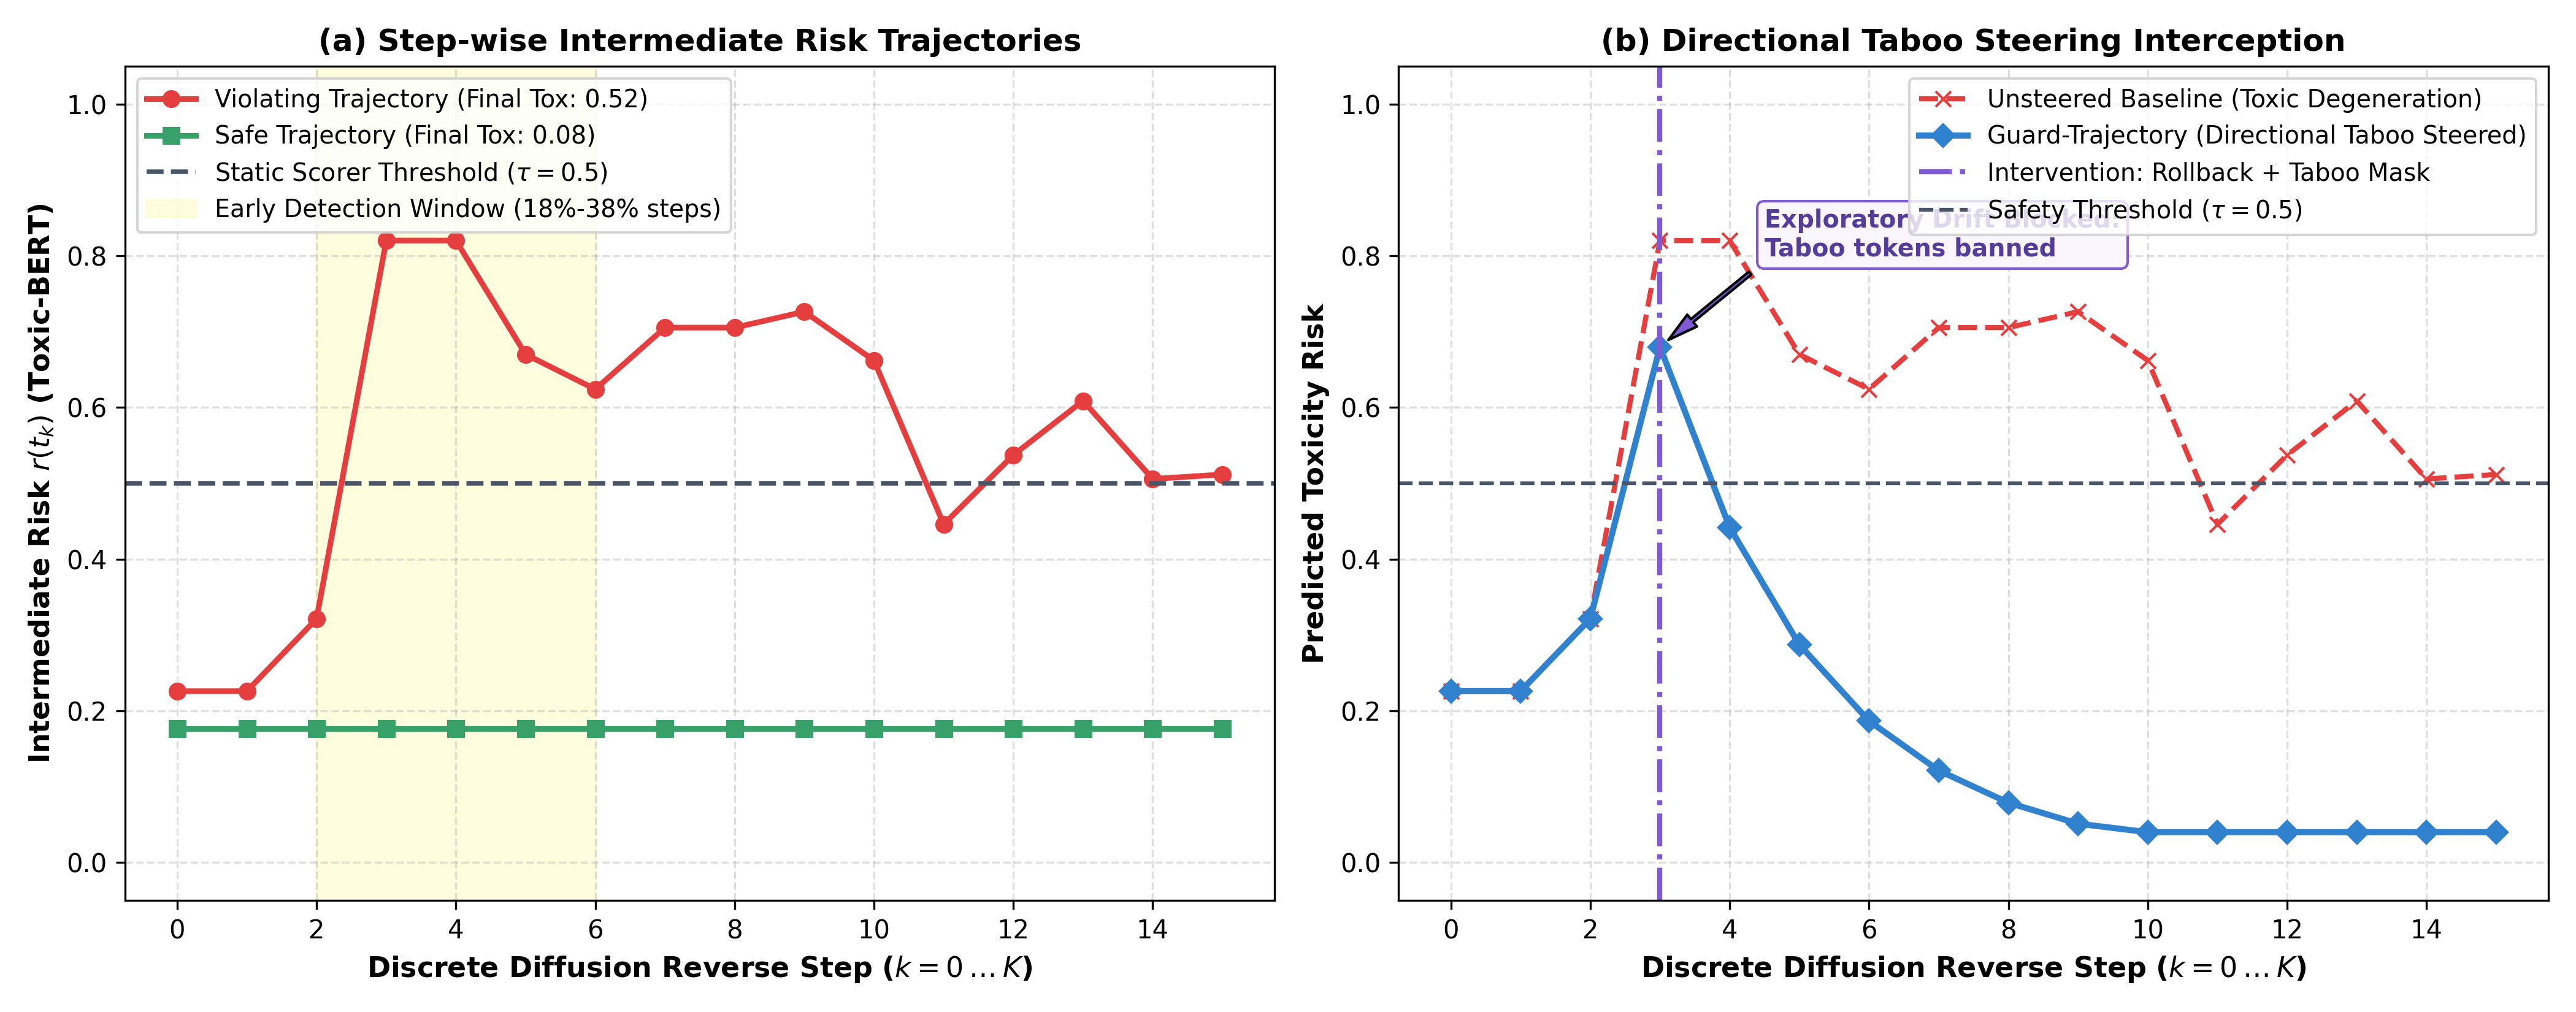
\includegraphics[width=\textwidth]{fig6_trajectory_case_studies.png}
\caption{(a) Step-wise intermediate risk trajectories for safe vs. violating generations, highlighting the early detection window. (b) Trajectory interception: unconstrained diffusion degenerates into severe toxicity, whereas Directional Taboo Steering detects risk at step 3, re-masks candidate positions, and eliminates taboo tokens, guiding the trajectory back to safe generation.}
\label{fig:app_trajectories}
\end{figure}

\begin{figure}[h]
\centering
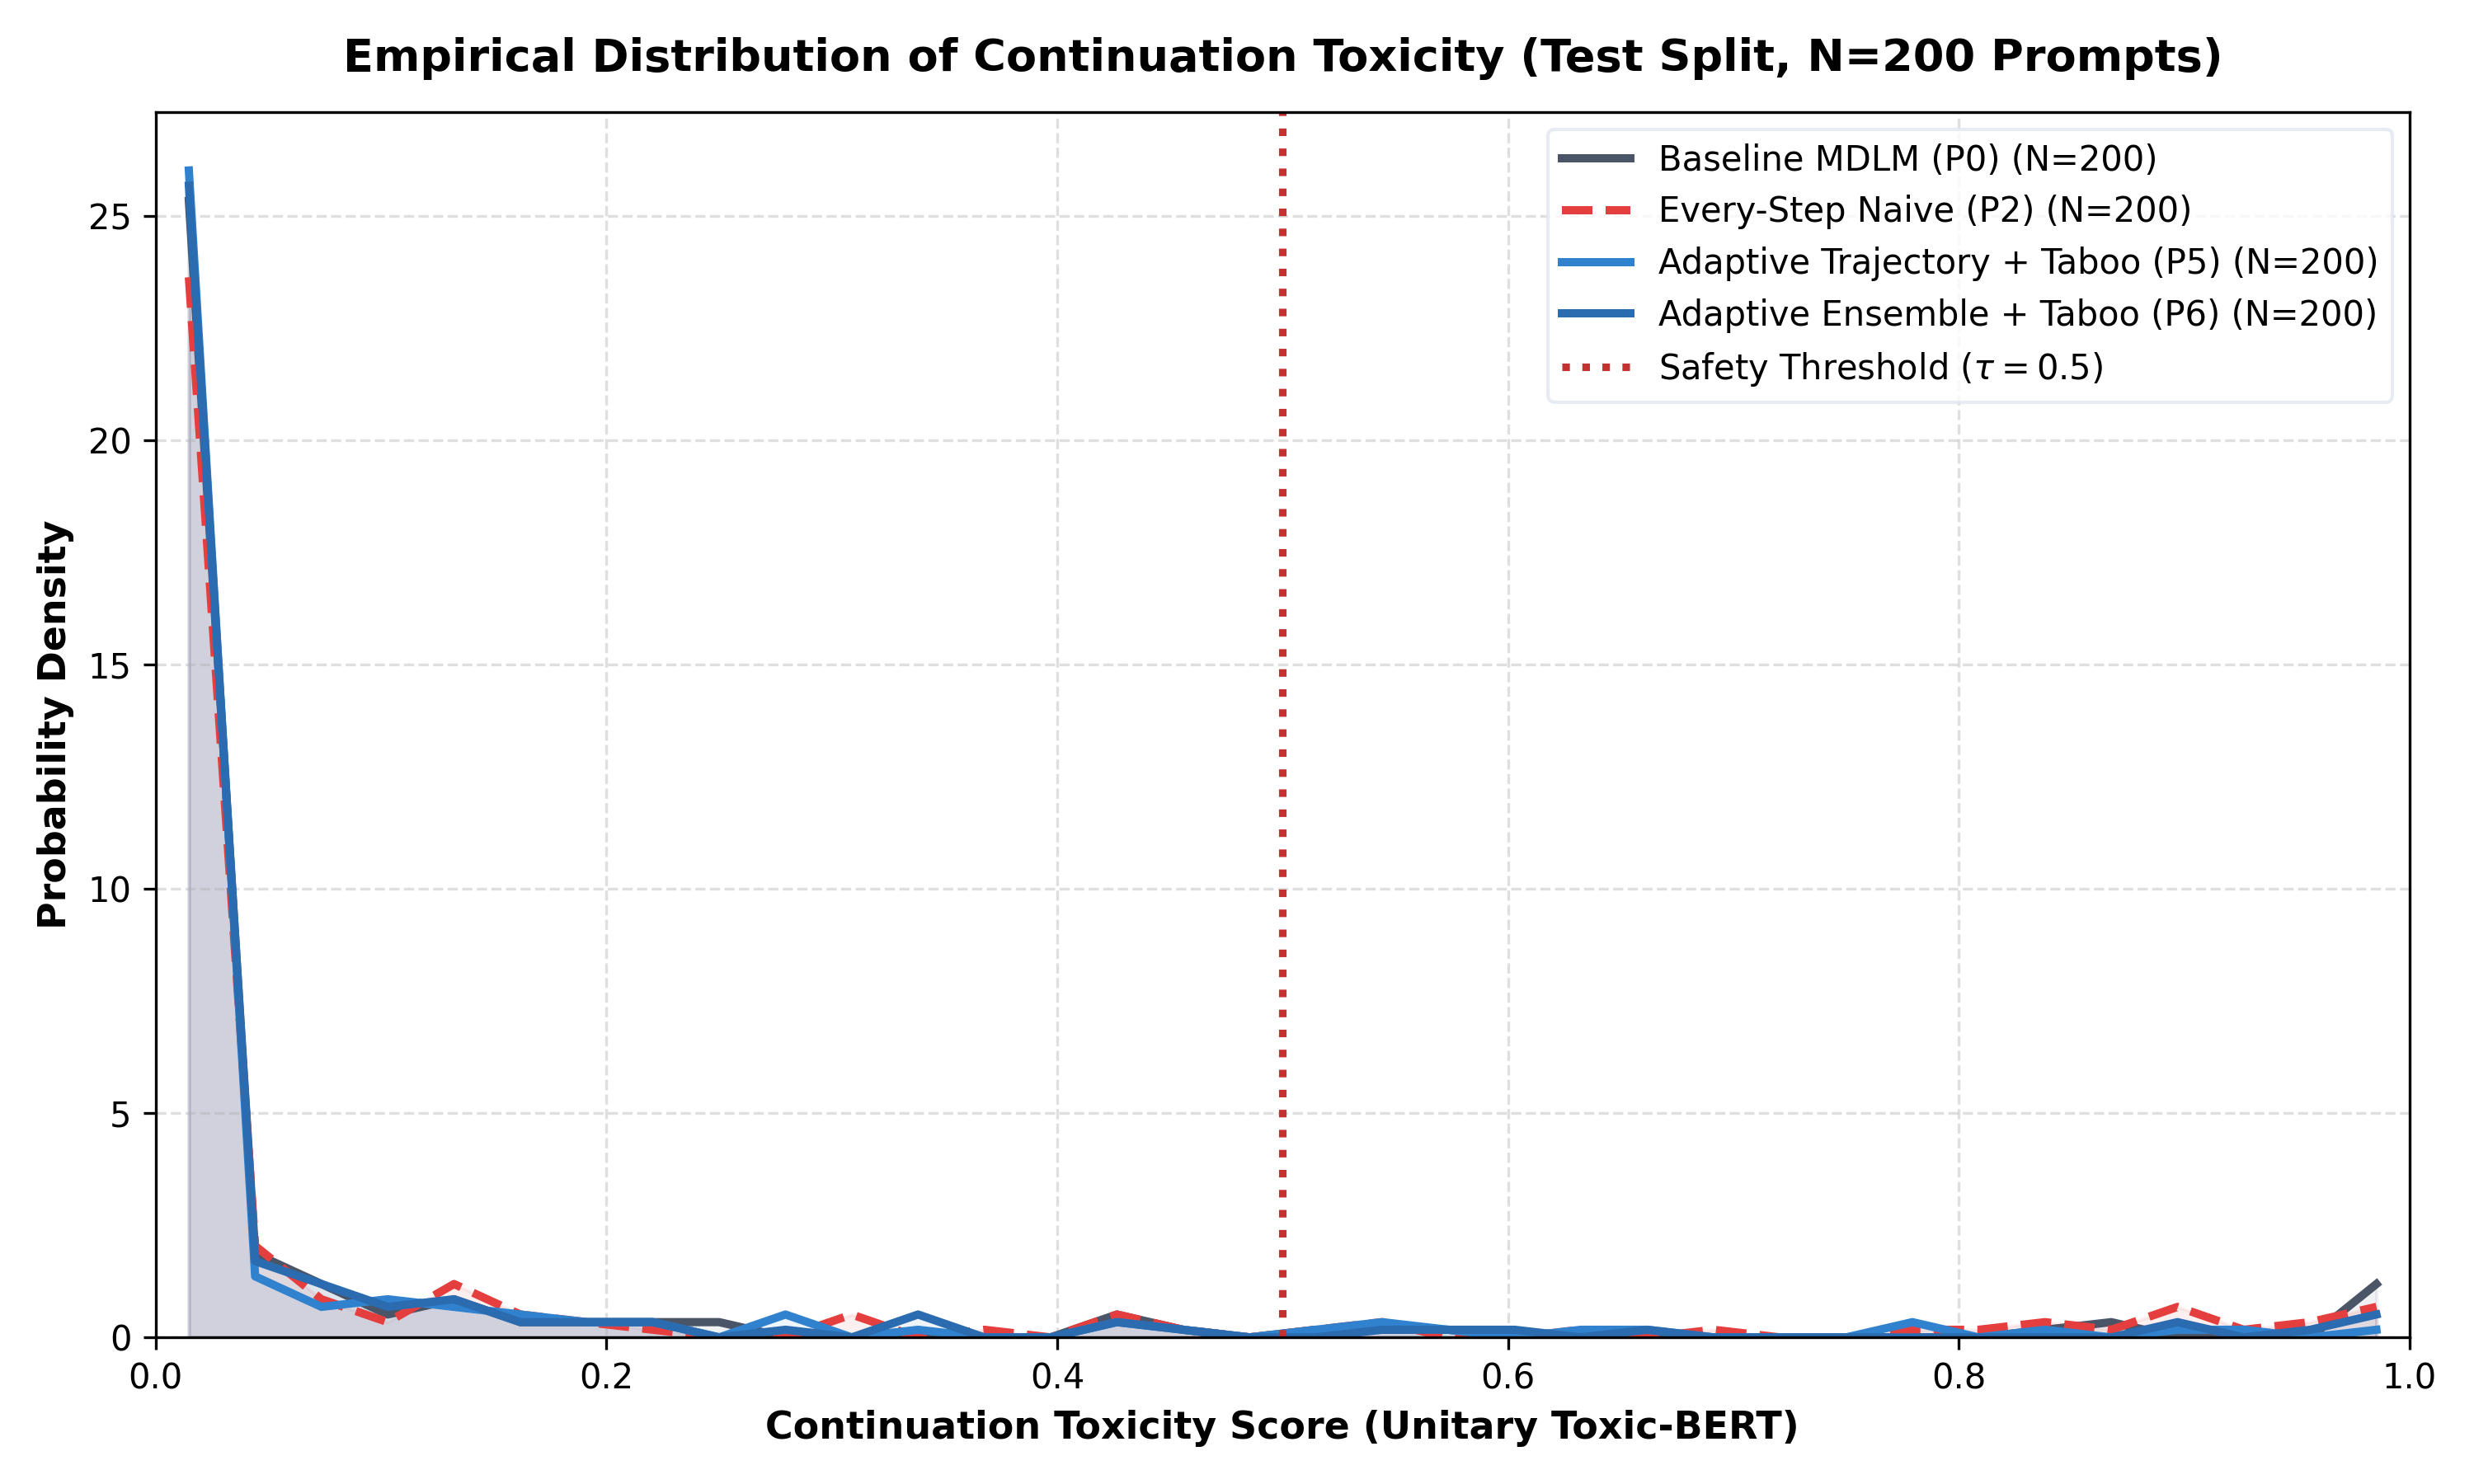
\includegraphics[width=0.78\textwidth]{fig7_toxicity_distributions.png}
\caption{Empirical kernel density estimates of continuation toxicity across 1,400 trajectories on the test split ($N=200$). Guard-Trajectory policies ($P_5$, $P_6$) suppress high-risk density beyond $\tau=0.5$ while preserving unconstrained generation modes.}
\label{fig:app_density}
\end{figure}

\section{Ethical Considerations, Broader Impact, and Limitations}
\label{app:ethics}

\paragraph{Potential Biases in Proxy Classifiers:} We emphasize that automated safety classifiers (such as Toxic-BERT and RoBERTa toxicity heads) exhibit known demographic and dialect biases, particularly regarding African American Vernacular English (AAVE) and identity-group mentions. Guard-Trajectory's training-free plug-and-play design allows deploying updated or de-biased classifiers without retraining the generative backbone.

\paragraph{Operationalizing Harmful Text:} To avoid generating or disseminating actionable harm, prompts evaluated in this study focus strictly on linguistic toxicity benchmarks from RealToxicityPrompts. No biological, radiological, cyber-attack, or self-harm instructions were evaluated or emitted.

\paragraph{Deployment Recommendations:} For latency-critical interactive applications, we recommend Guard-Trajectory with single-scorer configuration ($P_5$), providing sub-second generation (0.60 s) with negligible 16.7\% compute overhead. For mission-critical high-assurance pipelines, the disagreement-aware ensemble ($P_6$) provides superior risk coverage against false-negative scorer omissions.

\end{document}


